% ----------------------------------------------------
% Magic Comments for LaTeX-editors (TeXstudio, VSCode with LaTeX Workshop extension...)
% !TeX encoding = utf8
% !TeX spellcheck = de_DE
% !TeX program = pdflatex
% !BIB program = biber
% ----------------------------------------------------

% ----------------------------------------------------
% Load the HfTL-Thesis class
\documentclass[
% Select the main Language of your thesis here. Titlepage, captions and statement of authorship will change accordingly:
%
ngerman % - Deutsch (default)
% USenglish % - American english
% UKenglish % - British english
%
numeric % (default) use numeric citation style sorted by the occurence in text: [5]
% alphabetic % - use alphabetic citation style: [Lau95]
% authoryear % - use authoryear citation style: Laubach 1995
]{wbh-assignment}
% ----------------------------------------------------

% ----------------------------------------------------
% Load your own packages here
\usepackage{amsmath}
\usepackage{amsfonts}
\usepackage{amssymb}
\usepackage{graphicx}
\usepackage{scrlayer}
\usepackage{tabularx}
\usepackage{geometry}
\usepackage{setspace}
\usepackage[right]{eurosym}
%\usepackage[printonlyused]{acronym}
\usepackage{subfig}
\usepackage{floatflt}
% \usepackage[usenames,dvipsnames]{color}
\usepackage{colortbl}
\usepackage{paralist}
\usepackage{array}
%\usepackage{titlesec}
% \usepackage{parskip}
\usepackage[right]{eurosym}
%\usepackage{wrapfig}
% \usepackage[subfigure,titles]{tocloft}
\usepackage{helvet}
\usepackage{XCharter}
\usepackage{listings}
\usepackage{xcolor}
\usepackage{tcolorbox}
% \usepackage{enumitem}
% \usepackage{tikz}
% \usetikzlibrary{automata, positioning, arrows}

% Definition der gewünschten Rahmenfarbe mit Hex-Code
\definecolor{rahmenfarbe}{HTML}{d7005f}

% Definition des tcolorbox-Umfelds für Aufgabenstellungen
\newtcolorbox{aufgabenstellung}[1][]{%
  colback=white,  % Hintergrundfarbe
  colframe=rahmenfarbe,   % Rahmenfarbe
  title=Aufgabenstellung, % Titel der Box
  sharp corners,
  #1
}

\definecolor{ao(english)}{rgb}{0.0, 0.5, 0.0}

\lstset{
%	language=Prolog,
	basicstyle=\footnotesize,
	keywordstyle=\color{blue},
	commentstyle=\color{gray},
	stringstyle=\color{ao(english)},
	numbers=left,
	numberstyle=\tiny\color{gray},
	stepnumber=1,
	numbersep=5pt,
	backgroundcolor=\color{lightgray!20},
	frame=single,
	tabsize=2,
	captionpos=b,
	breaklines=true,
	breakatwhitespace=false,
	showspaces=false,
	showstringspaces=false,
	showtabs=false,
	morekeywords={:-},
}

% ----------------------------------------------------

% ----------------------------------------------------
% The document body. Start your work here.
\geometry{a4paper, top=25mm, left=30mm, right=40mm, bottom=25mm, headsep=10mm, footskip=12mm}

\renewcommand{\familydefault}{\sfdefault}

% ----------------------------------------------------
% Include own references
% \addbibresource{References/online.bib}
% \addbibresource{References/3gpp.bib}
% \addbibresource{References/etsi.bib}
% \addbibresource{References/itut.bib}
% \addbibresource{References/rfc.bib}
% \addbibresource{References/zotero.bib}
% \addbibresource{References/new.bib}
% \addbibresource{quellen.bib}
\addbibresource{references.bib}
\addbibresource{References/Embedded Software Engineering.bib}

% ----------------------------------------------------

% ----------------------------------------------------
% Load acronym definitions
%Eigene Definitionen
\newacronym{ftth}{FTTH}{Fiber To The Home}
\newacronym{fttc}{FTTC}{Fibre To The Curb}
\newacronym{fttb}{FTTB}{Fibre To The Building}
\newacronym{fttd}{FTTD}{Fibre To The Desk}
\newacronym{tkg}{TKG}{Telekommunikationsgesetz}
\newacronym{mbdc}{MBDC}{Minimum bidirectional net data rate capability}
\newacronym{pti}{PTI}{Produktion Technische Infrastruktur}
\newacronym{wfm t}{WFM T}{Workforce Management Technik}
\newacronym{kvz}{KVz}{Kabelverzweiger}
\newacronym{apl}{APL}{Abschlusspunkt Linientechnik}
\newacronym{mfg}{MFG}{Multifunktionsgehäuse}
\newacronym{nvt}{NVt}{Netzverteiler}
\newacronym{sve}{SVE}{Stromversorgungseinheit}
\newacronym{epk}{EPK}{Ereignisgesteuerte Prozesskette}
\newacronym{eepk}{eEPK}{erweiterte Ereignisgesteuerte Prozesskette}
\newacronym{epc}{EPC}{Event-driven Process Chain}
\newacronym{bpmn}{BPMN}{Business Process Model and Notation}
\newacronym{hk}{Hk}{Hauptkabel}
\newacronym{vzk}{Vzk}{Verzweigungskabel}
\newacronym{qk}{Qk}{Querkabel}
\newacronym{ovst}{OVSt}{Ortsvermittlungsstellen}
\newacronym{hvt}{HVt}{Hauptverteiler}
\newacronym{exif}{Exif}{Exchangeable Image File Format}
\newacronym{5g}{5G}{fünfte Generation [des Mobilfunks]}
\newacronym{gps}{GPS}{Global Positioning System}
\newacronym{onkz}{ONKZ}{Ortsnetzkennzahl}
\newacronym{asb}{ASB}{Anschlussbereich}
\newacronym{psl}{PSL}{Produktions-, Service-, Logistikprozesse}
\newacronym{pwa}{PWA}{Progressive Web App}
\newacronym{dsl}{DSL}{Digital Subscriber Line}
\newacronym{adsl}{ADSL}{Asymmetric Digital Subscriber Line}
\newacronym{hdsl}{HDSL}{High-Bit-Rate Digital Subscriber Line}
\newacronym{sdsl}{SDSL}{Symmetric Digital Subscriber Line}
\newacronym{vdsl}{VDSL}{Very-High-Bit-Rate Digital Subscriber Line}
\newacronym{fttx}{FTTx}{Fibre to the X}
\newacronym{diginetz}{DigiNetz}{Gesetz zur Erleichterung des Ausbaus digitaler Hochgeschwindigkeitsnetze}
\newacronym{atb-bestra}{ATB-BeStra}{Allgemeinen technischen Bestimmungen für die Benutzung von Strassen durch Leitungen und Telekommunikationslinien}
\newacronym{isdn}{ISDN}{Integrated Services Digital Network}
\newacronym{isdn d}{ISDN}{Integriertes Sprach- und Datennetz}
\newacronym{cn}{CN}{Corporate Network}
\newacronym{aps}{APS}{Arbeitsplatzsystem}
\newacronym{enas}{EnAS}{Energie-Anschluss-Säule}
\newacronym{bmvi}{BMVI}{Bundesministerium für Verkehr und digitale Infrastruktur}
\newacronym{gpon}{GPON}{Gigabit Passive Optical Network}
\newacronym{ptp}{PtP}{PtP-Ethernet}
\newacronym{olt}{OLT}{Optical Line Termination}
\newacronym{onu}{ONU}{Optical Network Unit}
\newacronym{ztv-tknetz}{ZTV-TKNetz}{Zusätzlichen Technischen Vertragsbedingungen der
Deutschen Telekom AG für Bauleistungen am Telekommunikationsnetz}
\newacronym{fstrg}{FStrG}{Bundesfernstraßengesetz}
\newacronym{dtag}{DTAG}{Deutschen Telekom AG}
\newacronym{mbfd}{MBfD}{Mehr Breitband für Deutschland}
\newacronym{html}{HTML}{HyperText Markup Language}
\newacronym{css}{CSS}{Cascading Style Sheets}
\newacronym{https}{HTTPS}{Hypertext Transfer Protocol Secure}

%Aus der Vorlage
\newacronym{3gpp}{3GPP}{Third Generation Partnership Project}

\newacronym{aaa}{AAA}{Authentication, Authorisation and Accounting}
\newacronym{aac-eld}{AAC-ELD}{Advanced Audio Coding-Enhanced Low Delay}
\newacronym{acr}{ACR}{Absolute Category Rating}
\newacronym{af}{AF}{Application Function}
\newacronym{agcf}{AGCF}{Access Gateway Control Function}
\newacronym{agch}{AGCH}{Access Grant Channel}
\newacronym{ajax}{AJAX}{Asynchronous JavaScript and XML}
\newacronym{amr}{AMR}{Adaptive Multi Rate}
\newacronym{amr-wb}{AMR-WB}{Adaptive Multirate-Wideband}
\newacronym{ape}{APE}{AJAX Push Engine}
\newacronym{api}{API}{Application Programming Interface}
%\acroplural{api}[APIs]{Application Programming Interfaces}
\newacronym{apn}{APN}{Access Point Name}
\newacronym{appserv}{AS}{Application Server}
\newacronym{armgw}{A/R-MGW}{Access/Residential-Media Gateway}
\newacronym{arvgw}{A/R-VGW}{Access/Residential-Voice over IP-Gateway}
\newacronym{as}{AS}{Access Stratum}
\newacronym{auc}{AuC}{Authentication Centre}
\newacronym{avp}{AVP}{Attribute-Value-Pairs}
\newacronym{ar}{AR}{Argumented Reality}
\newacronym{ad}{AD}{Activity Diagram}

\newacronym{bcch}{BCCH}{Broadcast Control Channel}
\newacronym{bgcf}{BGCF}{Breakout Gateway Control Function}
\newacronym{bsc}{BSC}{Base Station Controller}
\newacronym{bts}{BTS}{Base Transceiver Station}

\newacronym{ca}{CA}{Certificate Authority}
\newacronym{ca_mac}{CA}{Collision Avoidance}
\newacronym{camel}{CAMEL}{Customised Application for Mobile network Enhanced Logic}
\newacronym{cc}{CC}{Call Control, Country Code}
\newacronym{celp}{CELP}{Code-Excited Linear-Prediction}
\newacronym{celt}{CELT}{Constrained Energy Lapped Transform}
\newacronym{cli}{CLI}{Command Line Interface}
\newacronym{cm}{CM}{Connection Management}
\newacronym{cng}{CNG}{Comfort Noise Generation}
\newacronym{cod}{CoD}{Content on Demand}
\newacronym{cp}{CP}{Control Plane}
\newacronym{cpe}{CPE}{Customer-Premises Equipment}
\newacronym{cs}{CS}{Circuit Switched}
\newacronym{cs-acelp}{CS-ACELP}{Conjugate-Structure Algebraic-Code Excited Linear-Prediction}
\newacronym{cscf}{CSCF}{Call/Session Control Function}
\newacronym{csfb}{CSFB}{Circuit Switched Fallback}
\newacronym{csma}{CSMA}{Carrier Sense Medium Access}
%\newacronym{css}{CSS}{Cascading Style Sheets}
\newacronym{cps}{CPS}{Cyber-physische Systeme}

\newacronym{db}{DB}{Database}
\newacronym{dom}{DOM}{Document Object Model}
\newacronym{dscp}{DSCP}{Differentiated Services Code Points}
\newacronym{dtls}{DTLS}{Datagram Transport Layer Security}
\newacronym{dtx}{DTX}{Discontinuous Transmission}
\newacronym{dv}{DV}{Delay Variation}
\newacronym{dsgvo}{DSGVO}{Datenschutz-Grundverordnung}

\newacronym{e-rab}{E-RAB}{E-UTRAN Radio Access Bearer}
\newacronym{e-utran}{E-UTRAN}{Evolved UMTS Radio Access Network}
\newacronym{e2e}{E2E}{End-to-End}
\newacronym{edge}{EDGE}{Enhanced Data rates for GSM Evolution}
\newacronym{edss1}{EDSS1}{European Digital Subscriber System No. 1}
\newacronym{eir}{EIR}{Equipment Identity Centre, Equipment Identity Register}
%\newacronym{epc}{EPC}{Evolved Packet Core}
\newacronym{epg}{EPG}{Electronic Program Guide}
\newacronym{eps}{EPS}{Evolved Packet System}
\newacronym{etsi}{ETSI}{European Telecommunication Standards Institute}
\newacronym{etsi-tispan}{ETSI-TISPAN}{ETSI-Telecommunications and Internet converged Services and Protocols for AdvancedNetworking}

\newacronym{facch}{FACCH}{Fast Associated Control CHannel}
\newacronym{fb}{FB}{Fullband}
\newacronym{fcch}{FCCH}{Frequency Correction CHannel}
\newacronym{fec}{FEC}{Forward Error Correction}
\newacronym{fmc}{FMC}{Fixed Mobile Convergence}
\newacronym{fokus}{FOKUS}{Fraunhofer-Institut für Offene Kommunikationssysteme}
\newacronym{fr}{FR}{Full Rate}

\newacronym{geran}{GERAN}{GSM EDGE Radio Access Network}
\newacronym{ggsn}{GGSN}{Gateway GPRS Support Node}
\newacronym{gmm}{GMM}{GPRS Mobility Management}
\newacronym{gmsc}{GMSC}{Gateway MSC}
\newacronym{gprs}{GPRS}{General Packet Radio Service}
\newacronym{gsm}{GSM}{Global System for Mobile communications}
\newacronym{gsma}{GSMA}{GSM Association}
\newacronym{gtp}{GTP}{GPRS Tunneling Protocol}
\newacronym{gui}{GUI}{Graphical User Interface}
\newacronym{gw}{GW}{Gateway}

\newacronym{hd}{HD}{High Definition}
\newacronym{hlr}{HLR}{Home Location Register}
\newacronym{hr}{HR}{Half Rate}
\newacronym{hscsd}{HSCSD}{High-Speed Circuit-Switched Data}
\newacronym{hss}{HSS}{Home Subscriber Server}
\newacronym{html5}{HTML5}{Hypertext Markup Language Version 5}
\newacronym{http}{HTTP}{Hypertext Transfer Protocol}

\newacronym{iad}{IAD}{Integrated Access Device}
\newacronym{iana}{IANA}{Internet Assigned Numbers Authority}
\newacronym{ibcf}{IBCF}{Interconnection Border Control Function}
\newacronym{ibgf}{IBGF}{Interconnection Border Gateway Function}
\newacronym{ice}{ICE}{Interactive Connectivity Establishment}
\newacronym{i-cscf}{I-CSCF}{Interrogating-CSCF}
\newacronym{iesg}{IESG}{Internet Engineering Steering Group}
\newacronym{ietf}{IETF}{Internet Engineering Task Force}
\newacronym{imei}{IMEI}{International Mobile Equipment Identity}
\newacronym{ims}{IMS}{IP Multimedia Subsystem}
\newacronym{imscm}{IMSCM}{IMS-Client-Manager}
\newacronym{imsi}{IMSI}{International Mobile Subscriber Identity}
\newacronym{imssf}{IM-SSF}{IP Multimedia Service Switching Function}
\newacronym{imt}{IMT}{International Mobile Telecomunication}
\newacronym{inap}{INAP}{Intelligent Network Application Part}
\newacronym{ip}{IP}{Internet Protocol}
\newacronym{ip-can}{IP-CAN}{Internet Protocol- Connectivity Access Network}
\newacronym{ipdv}{IPDV}{IP Delay Variation}
\newacronym{iper}{IPER}{IP Packet Error Ratio}
\newacronym{iplr}{IPLR}{IP Packet Loss Ratio}
\newacronym{iptd}{IPTD}{IP Transfer Delay}
\newacronym{iptv}{IPTV}{Internet Protocol Television}
\newacronym{isc}{ISC}{IMS Service Control}
%\newacronym{isdn}{ISDN}{Integrated Services Digital Network}
\newacronym{iso/osi}{ISO/OSI}{Open System Interconnection/International Organization for Standardization}
\newacronym{isup}{ISUP}{ISDN User Part}
\newacronym{itu}{ITU}{International Telecommunication Union}
\newacronym{itu-t}{ITU-T}{International Telecommunications Union-Telecommunication Standardization Sector}
\newacronym{it}{IT}{Informationstechnologie}

\newacronym{json}{JSON}{JavaScript Object Notation}

\newacronym{ki}{KI}{Künstliche Intelligenz}

\newacronym{la}{LA}{Location Area}
\newacronym{label}{API}{Application Programming Interface}
\newacronym{lcp}{LCP}{Link Control Protocol}
\newacronym{llc}{LLC}{Logical Link Control}
\newacronym{lp}{LP}{Linear Prediction}
\newacronym{lte}{LTE}{Long Term Evolution}

\newacronym{m2m}{M2M}{Machine to Machine Communication}
\newacronym{mac}{MAC}{Medium Access Control}
\newacronym{mac_encryption}{MAC}{Message Authentication Code (encryption context)}
\newacronym{map}{MAP}{Mobile Application Part}
\newacronym{mcf}{MCF}{Media Control Function}
\newacronym{mdct}{MDCT}{Modified Discrete Cosine Transform}
\newacronym{mdf}{MDF}{Media Delivery Function}
\newacronym{mfv}{MFV}{Mehrfach Frequenz Wahlverfahren/Tonwahl}
\newacronym{mgc}{MGC}{Media Gateway Controler}
\newacronym{mgcf}{MGCF}{Media Gateway Control Function}
\newacronym{mgw}{MGW}{Media Gateway Function}
\newacronym{mime}{MIME}{Multipurpose Internet Mail Extensions}
\newacronym{mm}{MM}{Mobility Management}
\newacronym{mme}{MME}{Mobile Management Entity}
\newacronym{mos}{MOS}{Mean Opinion Score}
\newacronym{mrf}{MRF}{Multimedia Resource Function}
\newacronym{mrfc}{MRFC}{Multimedia Resource Function Controller}
\newacronym{mrfp}{MRFP}{Multimedia Resource Function Processor}
\newacronym{ms}{MS}{Mobile Station}
\newacronym{msc}{MSC}{Mobile Switching Centre}
\newacronym{msisdn}{MSISDN}{Mobile Subscriber ISDN Number}

\newacronym{n-pvr}{N-PVR}{Network-Personal Video Recorder}
\newacronym{napt}{NAPT}{Network Address and Port Translation}
\newacronym{nas}{NAS}{Non-Access Stratum}
\newacronym{nas_server}{NAS}{Network Access Server}
\newacronym{nass}{NASS}{Network Attachment Subsystem}
\newacronym{nat}{NAT}{Network Address Translation}
\newacronym{nb}{NB}{Narrowband}
\newacronym{nfv}{NFV}{Network Function Virtualization}
\newacronym{ngn}{NGN}{Next Generation Network}
\newacronym{nni}{NNI}{Network-Network Interface}
\newacronym{nodeb}{NodeB}{Funkbasisstation im UTRAN}
\newacronym{nsapi}{NSAPI}{Network Service Access Point Identifier}
\newacronym{ntba}{NTBA}{Network Termination for ISDN Basic rate Access / Netzterminator Basisanschluss}

\newacronym{osa}{OSA}{Open Service Access}
\newacronym{osascs}{OSA-SCS}{Open Service Access - Service Capability Server}
\newacronym{osgi}{OSGi}{Open Services Gateway initiative}
\newacronym{osi}{OSI}{Open System Interconnection}
\newacronym{ott}{OTT}{Over The Top Anwendungen}

\newacronym{p-cscf}{P-CSCF}{Proxy Call Session Control Function}
\newacronym{pcc}{PCC}{Policy and Charging Control}
\newacronym{pcef}{PCEF}{Policy Control Enforcement Function}
\newacronym{pch}{PCH}{Paging Channel}
\newacronym{pcrf}{PCRF}{Policy and Charging Rules Function}
\newacronym{pcu}{PCU}{Packet Control Unit}
\newacronym{pdn}{PDN}{Public Data Network, Packet Data Network}
\newacronym{pdn-gw}{PDN-GW}{Packet Data Network Gateway}
\newacronym{pelr}{PELR}{Packet Error Loss Rate}
\newacronym{pes}{PES}{PSTN/ISDN Emulation Subsystem}
\newacronym{pesq}{PESQ}{Perceptual Evaluation of Speech Quality}
\newacronym{pgw}{PGW}{Packet Data Network Gateway}
\newacronym{php}{PHP}{PHP: Hypertext Preprocessor}
\newacronym{plmn}{PLMN}{Public Land Mobile Network}
\newacronym{plr}{PLR}{Packet Loss Rate}
\newacronym{pnai}{PNAI}{Personal Network Administration Interface}
\newacronym{polqa}{POLQA}{Perceptual Objective Listening Quality Assessment}
\newacronym{pots}{POTS}{Plain Old Telephone System}
\newacronym{ppv}{PPV}{Pay-Per-View}
\newacronym{ps}{PS}{Packet Switched, Location Probability}
\newacronym{pss}{PSS}{PSTN/ISDN Simulation Subsystem}
\newacronym{pstn}{PSTN}{Public Switched Telephone Network}

\newacronym{qci}{QCI}{QoS Class Identifier}
\newacronym{qoe}{QoE}{Quality of Experience}
\newacronym{qos}{QoS}{Quality of Service}

\newacronym{ra}{RA}{Routing Area, Random mode request information field}
\newacronym{rab}{RAB}{Radio Access Bearer, Access Burst}
\newacronym{rat}{RAT}{Radio Access Technology}
\newacronym{rach}{RACH}{Random Access Channel}
\newacronym{racs}{RACS}{Resource Admission Control Subsystem}
\newacronym{radius}{RADIUS}{Remote Authentication Dial In User Service}
\newacronym{rcs}{RCS}{Rich Communication Suite}
\newacronym{rlc}{RLC}{Radio Link Control}
\newacronym{rnc}{RNC}{Radio Network Controller}
\newacronym{rpe-ltp}{RPE-LTP}{Regular Pulse Excitation - Long Term Prediction}
\newacronym{rr}{RR}{Radio Resources}
\newacronym{rrc}{RRC}{Radio Resource Control}
\newacronym{rtc}{RTC}{Real Time Communication}
\newacronym{rtcp}{RTCP}{RTP Control Protocol}
\newacronym{rtp}{RTP}{Realtime Transport Protocol}
\newacronym{rtsp}{RTSP}{Real-Time Streaming Protocol}
\newacronym{rtt}{RTT}{Round Trip Time}

\newacronym{sacch}{SACCH}{Slow Associated Control Channel}
\newacronym{sai}{SAI}{Service Attachment Information}
\newacronym{sapi}{SAPI}{Service Access Point Identifier}
\newacronym{scf}{SCF}{Service Control Function}
\newacronym{sch}{SCH}{Synchronisation Channel}
\newacronym{s-cscf}{S-CSCF}{Serving-CSCF}
\newacronym{sctp}{SCTP}{Stream Control Transmission Protocol}
\newacronym{sd}{SD}{Standard Definition}
\newacronym{sdcch}{SDCCH}{Stand-Alone Dedicated Control Channel}
\newacronym{sdf}{SDF}{Service Discovery Function}
\newacronym{sdma}{SDMA}{Space Division Multiple Access}
\newacronym{sdp}{SDP}{Session Description Protocol}
\newacronym{servgw}{ServGW}{Serving Gateway}
\newacronym{sgsn}{SGSN}{Serving GPRS Support Node}
\newacronym{sgw}{S-GW}{Signaling Gateway}
\newacronym{sigtran}{SIGTRAN}{ZGSNr.7 Signaling Transport Protocol Suite}
\newacronym{silk}{SILK}{SILK Speech codec}
\newacronym{sip}{SIP}{Session Initiation Protocol}
\newacronym{sipas}{SIP AS}{SIP Application Server}
\newacronym{slf}{SLF}{Subscriber Location Function}
\newacronym{sms}{SMS}{Short Message Service}
\newacronym{srtp}{SRTP}{Secure Real-Time Transport Protocol}
\newacronym{ss}{SS}{Supplementary Service}
\newacronym{sscon}{SSCON}{Session Controller}
\newacronym{ssf}{SSF}{Service Selection Function}
\newacronym{ssi}{SSI}{Service Selection Information}
\newacronym{ssrc}{SSRC}{Synchronization Source}
\newacronym{stun}{STUN}{Session Traversal Utilities for NAT}
\newacronym{swb}{SWB}{Super-Wideband}
\newacronym{smd}{SMD}{State Machine Diagram}

\newacronym{tch}{TCH}{Traffic Channel}
\newacronym{tcp}{TCP}{Transmission Control Protocol}
\newacronym{td}{TD}{Transfer Delay}
\newacronym{tdd}{TDD}{Time Division Duplex}
\newacronym{tispan}{TISPAN}{Telecommunications and Internet converged Services and Protocols for Advanced Networking}
\newacronym{tmsi}{TMSI}{Temporary Mobile Subscriber Identity}
\newacronym{tn}{TN}{Termination Node, Timeslot Number}
\newacronym{toc}{TOC}{Table-Of-Contents}
\newacronym{turn}{TURN}{Traversal Using Relays around NAT}
\newacronym{tv}{TV}{Television}
\newacronym{tsr}{TSR}{Traffic Sign Recognition}


\newacronym{ua}{UA}{User Agent}
\newacronym{udp}{UDP}{User Datagram Protocol}
\newacronym{ue}{UE}{User Equipment}
\newacronym{umts}{UMTS}{Universal Mobile Telecommunications System}
\newacronym{uni}{UNI}{User-Network Interface}
\newacronym{up}{UP}{User Plane}
\newacronym{upsf}{UPSF}{User Profile Server Function}
\newacronym{uri}{URI}{Uniform Resource Identifier}
\newacronym{url}{URL}{Uniform Resource Locator}
\newacronym{utran}{UTRAN}{Universal Terrestrial Radio Access Network}
\newacronym{ucd}{UCD}{Use Case Diagram}

\newacronym{vad}{VAD}{Voice Activity Dedection}
\newacronym{vbr}{VBR}{Variable Bit  Rate}
\newacronym{vgw}{VGW}{Voice over IP-Gateway}
\newacronym{vlc}{VLC}{VideoLan Client}
\newacronym{vod}{VoD}{Video on Demand}
\newacronym{voip}{VoIP}{Voice Over IP}
\newacronym{volga}{VoLGA}{Voice over LTE via Generic Access}
\newacronym{volte}{VoLTE}{Voice over LTE}

\newacronym{w3c}{W3C}{World Wide Web Consortium}
\newacronym{waf}{WAF}{WebRTC Authentication Function}
\newacronym{wb}{WB}{Wideband}
\newacronym{webrtc}{WebRTC}{Web Real-Time Communication}
\newacronym{wlan}{WLAN}{Wireless Local Area Network}
\newacronym{wqsf}{WQSF}{WebRTC QoS Signalling Function}
\newacronym{wwsf}{WWSF}{WebRTC Web Server Function}

\newacronym{xdsl}{xDSL}{any Digital Subscriber Line}
\newacronym{xml}{XML}{Extended MarkupLanguage}

\newacronym{zgs nr.7}{ZGS Nr.7}{Zentrales Zeichengabesystem Nr.7}
\newacronym{zd}{ZD}{Zustandsdiagramm}

\newacronym{ann}{ANN}{Artificial Neural Network}
\newacronym{mse}{MSE}{Mean Squared Error}
\newacronym{ea}{EA}{Evolutionäre Algorithmen}
\makenoidxglossaries % index acronyms
% ----------------------------------------------------

\begin{document}
% ----------------------------------------------------------------------------------------------------------
% Titelseite
% ----------------------------------------------------------------------------------------------------------
\newgeometry{margin=0.5in}
\thispagestyle{empty}
\begin{titlepage}
	\begin{center}
		\begin{figure}[h]
			\raggedleft
			\graphicspath{ {Images/} }
			
\includegraphics[scale=0.4]{logo_wbh.png}
		\end{figure}

		\vspace*{2cm}
		\Large \textbf{Studiengang:}\\
		\large \textbf{Embedded Systems and Digital Technologies}\\

		\vspace*{2cm}
		\LARGE \textbf{B-Aufgabe}\\
		\vspace*{0.5cm}
		\large B-EBF01-XX6-K02\\
		\vspace*{1cm}
		\Large \textbf{Embedded Software Engineering}\\

		\vspace*{2cm}
		\vfill

		\normalsize
		\newcolumntype{x}[1]{>{\raggedleft\arraybackslash\hspace{0pt}}p{#1}}
		\begin{tabular}{x{6cm}p{7.5cm}}
			\rule{0mm}{5ex}\textbf{Student:} & Kilian Vogler \newline kilian.vogler@gmail.com \\
			\rule{0mm}{5ex}\textbf{Matrikelnummer:} & 861105 \\
			\rule{0mm}{5ex}\textbf{Abgabedatum:} & 25.09.2025 \\
		\end{tabular}
	\end{center}
\end{titlepage}
\pagebreak
\restoregeometry

% ----------------------------------------------------------------------------------------------------------
% Verzeichnisse
% ----------------------------------------------------------------------------------------------------------

\onehalfspacing
\pagenumbering{Roman}
\tableofcontents %print the table of contents
\cleardoublepage

% ----------------------------------------------------------------------------------------------------------
% Inhalt
% ----------------------------------------------------------------------------------------------------------
% Abstände Überschrift

% Kopfzeile
\renewcommand{\sectionmark}[1]{\markright{#1}}
\renewcommand{\subsectionmark}[1]{}
\renewcommand{\subsubsectionmark}[1]{}

\onehalfspacing
\renewcommand{\thesection}{\arabic{section}}
\renewcommand{\theHsection}{\arabic{section}}
\setcounter{section}{0}
\pagenumbering{arabic}

% ----------------------------------------------------------------------------------------------------------
% Kapitel: Aufgabenstellung B-EBF01-XX6
% ----------------------------------------------------------------------------------------------------------
\section*{Aufgabenstellung B-EBF01-XX6}
\addcontentsline{toc}{section}{\protect\numberline{}Aufgabenstellung B-EBF01-XX6}
text
\cleardoublepage
text
\cleardoublepage
text
\cleardoublepage
% \setcounter{page}{1}

% ----------------------------------------------------------------------------------------------------------
% Kapitel 1: Zustandsdiagramm Scheibenwischersteuerung
% ----------------------------------------------------------------------------------------------------------
\section{Zustandsdiagramm Scheibenwischersteuerung}
\begin{aufgabenstellung}
Betrachten Sie die Steuerung durch Software eines Scheibenwischers. Der Scheibenwischer kann ausgeschaltet sein, oder auf der Stufe „einmal wischen“, Stufe 1 oder Stufe 2 sein.
Wenn die Option „Einmal wischen“ ausgewählt wird, wischt der Scheibenwischer nur einmal und schaltet sich wieder aus.
Der Fahrer hat die Möglichkeit ein automatisches Wischen der Windschutzscheiben auszuwählen, wenn es regnet.
Falls der Scheibenwischer ausgeschaltet ist, wird dieses automatische System aktiviert, sobald Regen auf die Windschutzscheibe fällt.
Erstellen Sie ein Zustandsdiagramm (state diagram) für den Scheibenwischer.
\end{aufgabenstellung}
\label{sec:state_diagram}

\vspace*{5mm}

Die grundlegenden Funktionen des Scheibenwischers sind in die folgenden Zustände unterteilt:

\begin{itemize}
    \item Aus (OFF)
    \item Einmal wischen (WIPE\_ONCE)
    \item Stufe 1 (LEVEL\_1)
    \item Stufe 2 (LEVEL\_2)
    \item Automatisch (AUTO)
\end{itemize}

Das folgende \ac{zd} (engl. \ac{smd}) modelliert die Zustände (\autoref{fig:state_diagram}) und die möglichen Übergänge zwischen ihnen.
Die mit \enquote{Driver} gekennzeichneten Übergänge zeigen an, dass der Fahrer manuell eine Änderung des Wischerzustands vornimmt.
Wohingegen die mit \enquote{Rain sensor} gekennzeichneten Übergänge anzeigen, dass die Änderung des Wischerzustands automatisch durch das System erfolgt, basierend auf dem Regensensor.

Das Diagramm ist in voller Größe in \autoref{fig:state_diagram} auf der nächsten Seite dargestellt.

\begin{figure}[htb!]
	\centering
	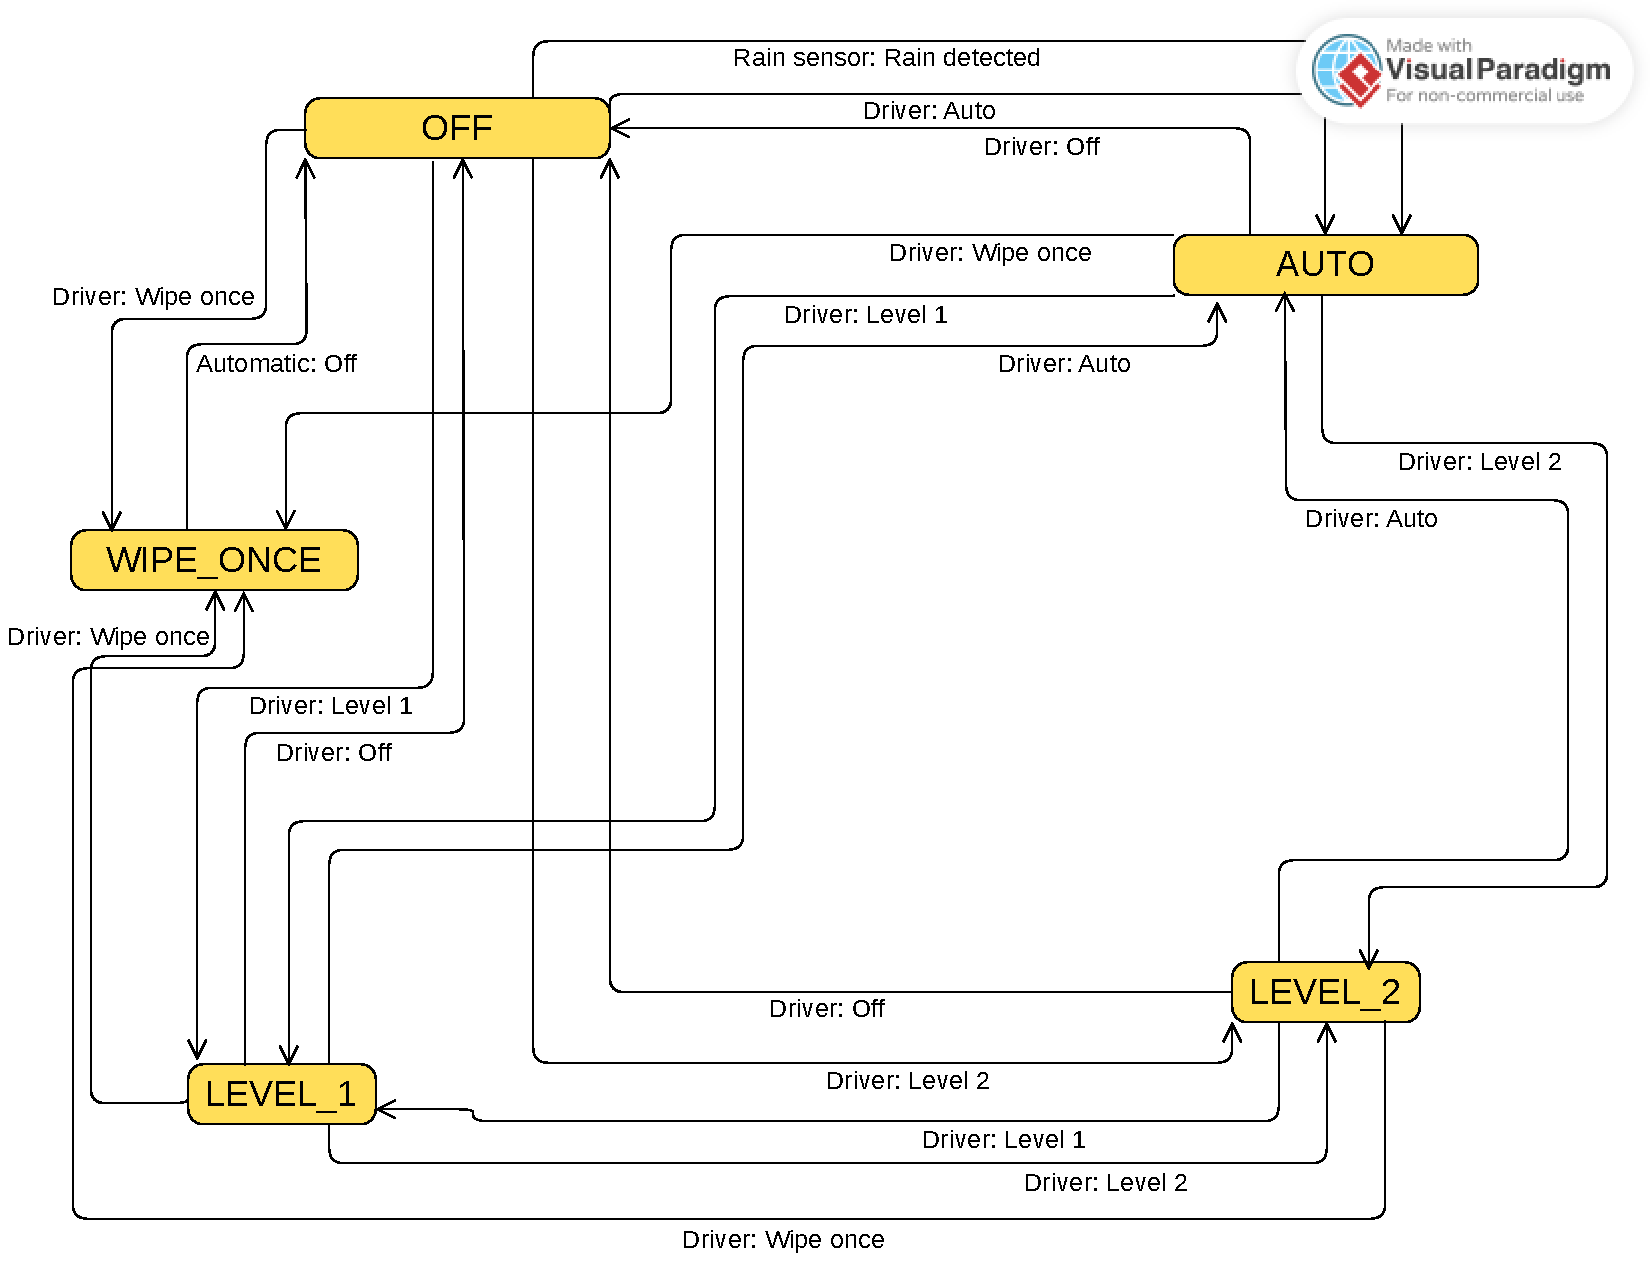
\includegraphics[width=1\linewidth]{Images/wiper_state_diagramm.pdf}
	\caption[\ac{zd} Scheibenwischer (eigene Darstellung mit \cite{VisualParadigmOnlineProduktivitatssuite})]{\ac{zd} Scheibenwischer (eigene Darstellung mit \cite{VisualParadigmOnlineProduktivitatssuite})}
	\label{fig:state_diagram}
\end{figure}

\clearpage

% ----------------------------------------------------------------------------------------------------------
% Kapitel 2: Akteure & Use-Case-Diagramm der Scheibenwischersoftware
% ----------------------------------------------------------------------------------------------------------
\section{Akteure \& Use-Case-Diagramm der Scheibenwischersoftware}

\subsection{Identifikation der Akteure}
\begin{aufgabenstellung}
Was sind Akteure und wie interagieren sie mit dem zu entwickelnden System?
\end{aufgabenstellung}

\vspace*{5mm}

Für das in \autoref{sec:state_diagram} betrachtete Scheibenwischersystem lassen sich die folgenden Akteure und deren Interaktionen mit dem System identifizieren:

\textbf{Akteure:}
\begin{itemize}
  \item \textbf{Fahrer / \enquote{Driver} (primärer Akteur):} \\
        wählt \glqq Aus\grqq, \glqq Einmal\grqq, \glqq Stufe 1\grqq, \glqq Stufe 2\grqq{} oder \glqq Auto\grqq.
  \item \textbf{Regensensor / \enquote{Rain sensor} (sekundärer Akteur):} \\
        liefert Information \glqq Regen erkannt / kein Regen\grqq{} sowie die \glqq Intensität des Regens\grqq.
\end{itemize}

\vspace*{5mm}

\textbf{Interaktion:}
\begin{itemize}
  \item Der Fahrer löst durch Eingaben Zustandswechsel des Wischers aus.
  \item Der Sensor interagiert automatisch und triggert Zustandswechsel im Automatikmodus und passt die Wischgeschwindigkeit an die Regenintensität an.
  \item Das System reagiert, indem es die Wischermotoren steuert und die gewünschte Funktion ausführt. Sowie schaltet sich bei \glqq Einmal wischen\grqq{} nach einem Zyklus wieder aus.
\end{itemize}


\subsection{Use-Case-Diagramm: Scheibenwischersoftware}
\begin{aufgabenstellung}
Erstellen Sie ein Anwendungsfalldiagramm (use-case diagramm) der Steuerungssoftware des Scheibenwischers in dieser Form (nur als Beispiel, das nichts über die Zahl der Use Cases und Akteure im gegebenen Fall aussagt): Der Regensensor sollte als Akteur modelliert werden.
\end{aufgabenstellung}

\vspace*{5mm}

Im folgenden Anwendungsfalldiagramm (engl. \ac{ucd}) sind die Akteure Fahrer (\enquote{Driver}) und Regensensor (\enquote{Rain sensor}) sowie deren Interaktionen mit dem Scheibenwischersystem (Windshield wiper software) in \autoref{fig:use_case_diagram} dargestellt.

\vspace*{5mm}

\begin{figure}[htb!]
	\centering
	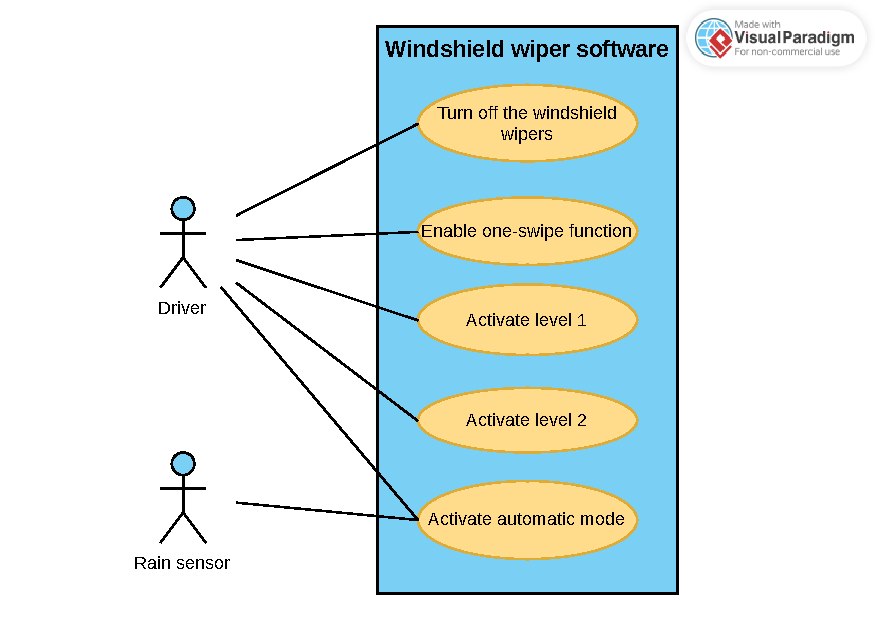
\includegraphics[width=1\linewidth]{Images/use_case_diagramm.pdf}
	\caption[\ac{ucd} Scheibenwischer (eigene Darstellung mit \cite{VisualParadigmOnlineProduktivitatssuite})]{\ac{ucd} Scheibenwischer (eigene Darstellung mit \cite{VisualParadigmOnlineProduktivitatssuite})}
	\label{fig:use_case_diagram}
\end{figure}

\clearpage

% ----------------------------------------------------------------------------------------------------------
% Kapitel 3: Aktivitätsdiagramm: Automatischer Scheibenwischerbetrieb
% ----------------------------------------------------------------------------------------------------------
\section{Aktivitätsdiagramm: Automatischer Scheibenwischerbetrieb}

\begin{aufgabenstellung}
Erstellen Sie ein UML-Aktivitätsdiagramm (Activity Diagram) für den Scheibenwischer für das folgende Szenario:
Der Scheibenwischer wird von Motoren angetrieben und seine Geschwindigkeit über einen Regensensor reguliert. Nehmen Sie an, dass das automatische Wischen schon eingeschaltet ist.
\end{aufgabenstellung}

\vspace*{5mm}

Im UML-Aktivitätsdiagramm (engl. \ac{ad}) in \autoref{fig:activity_diagram} ist der Ablauf des automatischen Scheibenwischerbetriebs modelliert.
Die Intensität des Regens ist in der Darstellung in die Zustände \enquote{kein Regen}, \enquote{leichter Regen}, \enquote{mäßiger Regen} und \enquote{starker Regen} unterteilt.
Es wurde auch die manuelle Abschaltung des Scheibenwischers berücksichtigt.
Nach einem Zeitintervall wird der Regensensor erneut abgefragt, um die Wischgeschwindigkeit entsprechend der aktuellen Regenintensität anzupassen.

Das UML-Aktivitätsdiagramm ist in voller Größe in \autoref{fig:activity_diagram} auf der nächsten Seite dargestellt.

\begin{figure}[htb!]
	\centering
	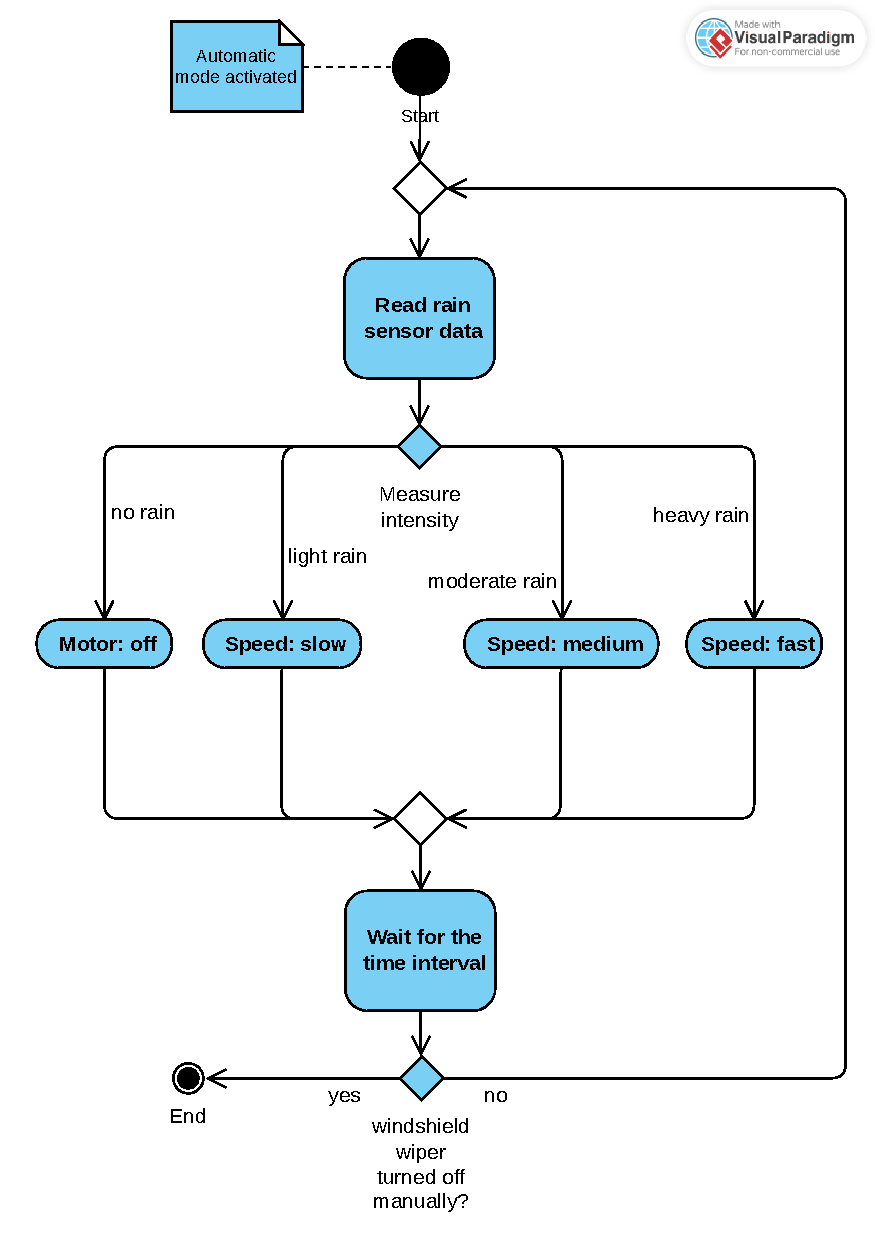
\includegraphics[width=1\linewidth]{Images/activity_diagramm.pdf}
	\caption[UML-\ac{ad} Scheibenwischer (eigene Darstellung mit \cite{VisualParadigmOnlineProduktivitatssuite})]{UML-\ac{ad} Scheibenwischer (eigene Darstellung mit \cite{VisualParadigmOnlineProduktivitatssuite})}
	\label{fig:activity_diagram}
\end{figure}

\clearpage

% ----------------------------------------------------------------------------------------------------------
% Kapitel 4: Nebenläufigkeit eingebetteter Systeme
% ----------------------------------------------------------------------------------------------------------
\section{Nebenläufigkeit eingebetteter Systeme}

\subsection{Inhärente Nebenläufigkeit eingebetteter Systeme}
\begin{aufgabenstellung}
Erläutern Sie, warum eingebettete Systeme inhärent nebenläufig sind und warum dies einen Grund für ihre hohe Entwurfskomplexität darstellt.
\end{aufgabenstellung}

\vspace*{5mm}

Eingebettete Systeme sind inhärent nebenläufig, da sie simultan auf verschiedene asynchrone Ereignisse reagieren müssen.
Dies zeigt sich im Scheibenwischersystem: Während das System kontinuierlich Regensensordaten auswertet und die Motorgeschwindigkeit entsprechend anpasst, muss es gleichzeitig auf manuelle Benutzereingaben reagieren können.
Der Regensensor arbeitet in regelmäßigen Intervallen, unabhängig von der Motorsteuerung oder Benutzereingaben.
Hinzu kommt eine interrupt gesteuerte Architektur, bei der externe Events wie Sensormessungen oder Timer-Interrupts jederzeit eintreten und die Hauptausführung unterbrechen können.

Die hohe Entwurfskomplexität entsteht durch Race Conditions beim gleichzeitigen Zugriff auf gemeinsame Systemzustände und die Notwendigkeit deterministischer Echtzeitreaktionen trotz paralleler Prozesse und die schwierige Vorhersagbarkeit des Systemverhaltens.
Darüber hinaus erfordert die Beschränkung auf begrenzte Ressourcen, wie CPU-Zeit, Speicher und Energie, eine sorgfältige Priorisierung und Synchronisation der Tasks.
Debugging wird zudem erschwert, da timing abhängige Fehler oft nicht reproduzierbar sind und spezielle Analysetools benötigt werden, um Race Conditions oder Deadlocks aufzuspüren \cite{cummingsManagingConcurrencyComplex, ConcurrencyInterruptsMicrocontrollers}.

\newpage

\subsection{POSIX Threads: Umsetzung der Nebenläufigkeit}
\begin{aufgabenstellung}
Nebenläufige Tasks werden in der Programmiersprache C mithilfe von POSIX Threads implementiert. Erklären Sie kurz, wie Threads die Nebenläufigkeit implementieren.
\end{aufgabenstellung}

\vspace*{5mm}

POSIX Threads implementieren Nebenläufigkeit durch die Aufteilung der Programmlogik in mehrere parallel ausführbare Einheiten.
Jeder Thread erhält einen eigenen Ausführungskontext: Stack, Programmzähler, Register, während alle Threads denselben Adressraum teilen.
Das ermöglicht effizienten Datenaustausch über gemeinsame Variablen \cite{LinuxTutorialPOSIX}.

Das Betriebssystem verwendet präemptives Scheduling, um Threads zeitscheibenbasiert oder prioritätsgesteuert auf verfügbare CPU-Kerne zu verteilen.
Moderne pthread-Implementierungen nutzen Kernel-Level-Threads für echte Parallelität auf Mehrkernsystemen.
Synchronisationsmechanismen wie Mutexes und Condition Variables koordinieren den Zugriff auf gemeinsame Ressourcen.

\newpage

\subsection{Zusätzliche Thread-Funktionen im Scheibenwischersystem}
\begin{aufgabenstellung}
Betrachten Sie wieder das Scheibenwischersystem. Das Folgende zeigt eine Funktion (im Pseudocode), die ein Thread ausführen kann.
Geben Sie zwei weitere Funktionen an, die beim Scheibenwischersystem als Threads ausgeführt werden können.
\end{aufgabenstellung}

\vspace*{5mm}

Im Folgenden zwei Threads für das Scheibenwischersystem. Zum einen der Regensensor-Thread und der Motorsteuerungs-Thread. \newline
Mit dem Regensensor-Thread wird die Regenintensität kontinuierlich überwacht und die Wischgeschwindigkeit entsprechend angepasst.

\vspace*{5mm}

\begin{lstlisting}[language=C, caption={Regensensor-Thread}]
void* RainSensor_Thread() {
    while(1) {
        int rainIntensity = readRainSensor();

        int wiperSpeed;
        if(rainIntensity == 0) {
            wiperSpeed = OFF;
        }
        else if(rainIntensity <= LIGHT) {
            wiperSpeed = SLOW;
        }
        else if(rainIntensity <= MODERATE) {
            wiperSpeed = MEDIUM;
        }
        else {
            wiperSpeed = FAST;
        }

        writeSpeedToBuffer(wiperSpeed);

        waitSamplingInterval();

        if(isSystemManuallyOff()) break;
    }
    return NULL;
}
\end{lstlisting}

\newpage

Mit dem Motorsteuerungs-Thread wird die Wischgeschwindigkeit basierend auf den Daten des Regensensors eingestellt und der Wischzyklus gestartet.
Es wird zudem auch nach dem Wischzyklus überprüft, ob das System manuell ausgeschaltet wurde.

\vspace*{5mm}

\begin{lstlisting}[language=C, caption={Motorsteuerungs-Thread}]
void* MotorControl_Thread() {
    while(1) {
        int currentSpeed = readSpeedFromBuffer();

        switch(currentSpeed) {
            case OFF:
                stopMotor();
                break;
            case SLOW:
                setMotorSpeed(SLOW_VALUE);
                startWipeCycle();
                break;
            case MEDIUM:
                setMotorSpeed(MEDIUM_VALUE);
                startWipeCycle();
                break;
            case FAST:
                setMotorSpeed(FAST_VALUE);
                startWipeCycle();
                break;
        }

        if(isSystemManuallyOff()) {
            stopMotor();
            break;
        }

        usleep(MOTOR_CYCLE_DELAY);
    }
    return NULL;
}
\end{lstlisting}

\newpage

\subsection{Kommunikation und Synchronisation der Threads}
\begin{aufgabenstellung}
Beschreiben Sie, warum die Threads miteinander kommunizieren oder sich synchronisieren müssen. Geben Sie auch an, wie Sie die Kommunikation oder Synchronisation implementieren würden (nur das Mittel, nicht den Code).
\end{aufgabenstellung}

\vspace*{5mm}

Die Threads müssen miteinander kommunizieren, weil sie gemeinsame Daten austauschen und koordiniert arbeiten müssen.
Der Regensensor-Thread bestimmt basierend auf Sensormessungen die erforderliche Motorgeschwindigkeit, die der Motorsteuerungs-Thread umsetzen muss.
Ohne Kommunikation könnte der Motor nicht auf Änderungen der Regenintensität reagieren.

Die Synchronisation ist erforderlich, um Race Conditions zu vermeiden.
Wenn beide Threads gleichzeitig auf den gemeinsamen Geschwindigkeitspuffer zugreifen, während der Regensensor-Thread eine neue Geschwindigkeit schreibt und der Motorsteuerungs-Thread diese liest, können inkonsistente Daten entstehen.
Dies könnte zu unvorhersagbarem Motorverhalten oder Systemfehlern führen.
Um dies zu verhindern, gibt es die folgenden Mechanismen in der Implementierung:

\begin{itemize}
  \item \textbf{Mutex (pthread\_mutex\_t)}: Schützt den kritischen Abschnitt beim Zugriff auf den gemeinsamen Geschwindigkeitspuffer und verhindert gleichzeitige Lese-/Schreibzugriffe.
  \item \textbf{Condition Variables (pthread\_cond\_t)}: Signalisieren Ereignisse zwischen den Threads, z.\,B. wenn der Regensensor-Thread eine neue Geschwindigkeit ermittelt hat oder wenn das System manuell ausgeschaltet wird.
  \item \textbf{Shared Buffer}: Ein geschützter Speicherbereich zur Übertragung der Geschwindigkeitswerte zwischen den Threads.
  \item \textbf{Atomic Variables}: Für einfache Statusflags wie den manuellen Ausschaltbefehl, um lockfreie Synchronisation zu ermöglichen.
\end{itemize}

Diese Mechanismen gewährleisten Datenintegrität trotz paralleler bzw. überlappender Ausführung der Threads.

% ----------------------------------------------------------------------------------------------------------
% Kapitel 5: Echtzeitsysteme & Verkehrszeichenerkennung
% ----------------------------------------------------------------------------------------------------------
\section{Echtzeitsysteme \& Verkehrszeichenerkennung}

\subsection{Echtzeitsystem-Analyse: Scheibenwischer}
\begin{aufgabenstellung}
Ist der Scheibenwischer in Aufgabe 1 ein Echtzeitsystem? Begründen Sie Ihre Antwort?
\end{aufgabenstellung}

% \vspace*{5mm}

Der Scheibenwischer aus \autoref{sec:state_diagram} ist ein Echtzeitsystem, weil er zeitkritisch auf äußere Ereignisse, wie hier das Fallen von Regen, reagieren muss.
Die Steuerungssoftware darf die Aktivierung des Wischers bei Regen nicht zu stark verzögern, dass die Sicht des Fahrers zu sehr beeinträchtigt wird.
Hier kann eine späte Reaktion zu Gefährdungen führen und es müssen alle Rechen- und Sensorzugriffe innerhalb definierter Fristen abgeschlossen sein.
Da jedoch gelegentliche geringfügige Verzögerungen um wenige Millisekunden nicht unmittelbar katastrophale Folgen haben, handelt es sich um ein weiches Echtzeitsystem \cite{HowAchieveDeterministic}.

\subsection{Beispielhafte Anwendungen der Verkehrszeichenerkennung}
\begin{aufgabenstellung}
Beschreiben Sie mithilfe von Beispielen, wie ein Verkehrszeichenerkennungssystem verwendet werden könnte.
\end{aufgabenstellung}

% \vspace*{5mm}

Verkehrszeichenerkennungssysteme (\ac{tsr}) analysieren in Echtzeit Kamerabilder, um Verkehrszeichen zu identifizieren und deren Information an den Fahrer oder Fahrassistenzsysteme zu übermitteln.
Beispiele hierfür sind die folgenden Systeme:
\begin{itemize}
  \item Anzeige der zulässigen Höchstgeschwindigkeit im Kombiinstrument oder Head-Up-Display, sowie Warnung bei Überschreitung.
  \item Automatische Anpassung der Geschwindigkeit im adaptiven Tempomaten basierend auf erkannten Geschwindigkeitsbegrenzungen.
\end{itemize}

\subsection{Echtzeitfähigkeit und Klassifizierung von Verkehrszeichenerkennungssystemen}
\begin{aufgabenstellung}
Erläutern Sie, warum Verkehrszeichenerkennungssysteme echtzeitfähig sein müssen. Handelt es sich um harte Echtzeitsysteme? Begründen Sie Ihre Antwort.
\end{aufgabenstellung}

Verkehrszeichenerkennung muss echtzeitfähig sein, weil erkannte Informationen nur innerhalb eines engen Zeitfensters relevant sind.
Wird ein Tempolimit zu spät erkannt, kann das Assistenzsystem nicht rechtzeitig die Fahrzeuggeschwindigkeit anpassen und der Fahrer könnte in eine Gefahrenlage geraten bzw. an der Stelle mit Beginn der Geschwindigkeitsbegrenzung noch eine zu hohe Geschwindigkeit fahren.

Da in diesem Beispiel eine einzelne Fristverletzung typischerweise nicht sofort katastrophal ist, es könnte ein verpasstes Schild zu Komforteinbußen oder Bußgeldrisiken führen, wird \ac{tsr} üblicherweise als weiches Echtzeitsystem klassifiziert.
Harte Echtzeitsysteme erfordern, dass jede Deadline ohne Ausnahme absolut eingehalten wird, was hier nicht in gleicher Weise gefordert ist \cite{HowAchieveDeterministic}.
Ein Beispiel für ein hartes Echtzeitsystem im Bereich der Fahrzeugtechnik wäre ein Airbag-Steuergerät, bei dem eine Fristverletzung zu lebensbedrohlichen Folgen führen kann.

\clearpage

\cleardoublepage

\appendix
\pagenumbering{Roman}
\setcounter{page}{1}

% Redefine \chapter* to not cause a page break
\makeatletter
\renewcommand\chapter{\@startsection{chapter}{0}{\z@}%
	{-3.5ex \@plus -1ex \@minus -.2ex}%
	{2.3ex \@plus.2ex}%
	{\normalfont\Large\bfseries}}
\makeatother

\begingroup
\raggedright
\printbibliography
\endgroup

\nopagebreak
\printnoidxglossary[type=\acronymtype] % print the list of abbreviations

\nopagebreak
\listoffigures % print the list of figures

% \nopagebreak
% \listoftables % print the list of tables

\nopagebreak
\lstlistoflistings % print the list of source codes

% \clearpage
% \makedeclarationofauthorship % print the declaration of authorship

\end{document}